

\documentclass[11pt]{beamer}

\usetheme{Madrid}
\usecolortheme{seahorse}
\setbeamertemplate{navigation symbols}{}

\usepackage[utf8]{inputenc}
\usepackage[T1]{fontenc}
\usepackage[ngerman,english]{babel}
\usepackage{amsmath,amssymb,bm,mathtools}
\usepackage{graphicx}
\usepackage{booktabs}
\usepackage{microtype}

\newcommand{\E}{\mathbb E}
\newcommand{\Var}{\operatorname{Var}}
\newcommand{\sigmoid}{\sigma}

\title[Spatial Poisson Fields]{From Point Events to Posterior Fields}
\author[T. Luhdo]{Toni Luhdo}
\institute[UP]{University of Potsdam}
\date[SFB Talk 2026]{SFB / Working Group Talk}

\AtBeginSection[]{
\begin{frame}{Outline}
\tableofcontents[currentsection]
\end{frame}
}

\begin{document}

\begin{frame}
\titlepage
\end{frame}

\begin{frame}{Roadmap}
\tableofcontents
\end{frame}

% -------------------------------------------------
\section{Motivation}

\begin{frame}{Spatial Event Data}
Typical examples:
\begin{itemize}
\item Earthquakes
\item Photon arrivals in imaging
\item Disease outbreaks
\item Crime hotspots
\end{itemize}

Observed data are often \textbf{point events} in space.

Goal: infer an underlying smooth intensity field.
\end{frame}

\begin{frame}{Synthetic Point Catalog}
\begin{center}
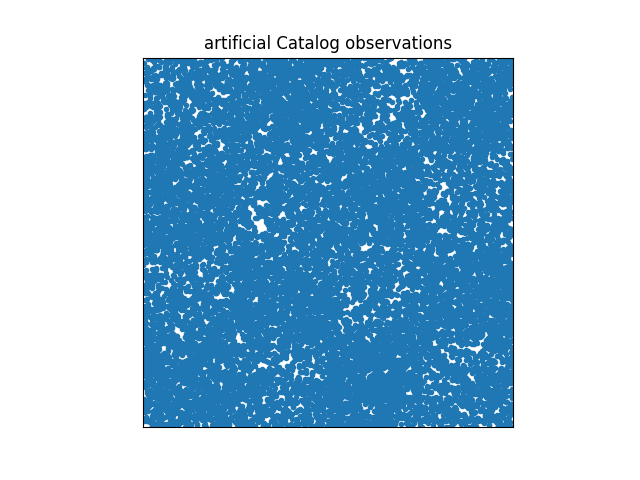
\includegraphics[width=0.72\textwidth]{figures/Figure_3.png}
\end{center}

We observe only events, not the true latent rate.
\end{frame}

% -------------------------------------------------
\section{Generative Model}

\begin{frame}{Latent Gaussian Field}
We introduce a latent spatial field:
\[
f \sim \mathcal N(\mu,\Sigma)
\]

where $\Sigma$ encodes spatial correlation.

Interpretation:
\begin{itemize}
\item nearby cells are correlated
\item smoothness is controlled by the covariance kernel
\item prior information enters naturally
\end{itemize}
\end{frame}

\begin{frame}{From Latent Field to Poisson Rate}
Rates must be positive. We use:
\[
\lambda_i = \lambda\,\sigmoid(f_i),
\qquad
\sigmoid(x)=\frac{1}{1+e^{-x}}
\]

Then:
\[
0 < \lambda_i < \lambda
\]

Advantages:
\begin{itemize}
\item positivity
\item bounded intensity
\item numerically stable inference
\end{itemize}
\end{frame}

\begin{frame}{Induced Prior on Intensity}
\begin{center}

\includegraphics[width=0.78\textwidth]{figures/Figure_1.png}
\end{center}

A Gaussian prior on $f$ induces a non-Gaussian prior on $\lambda_i$.
\end{frame}

\begin{frame}{Synthetic Example I: Structured Rate Field}
\begin{center}
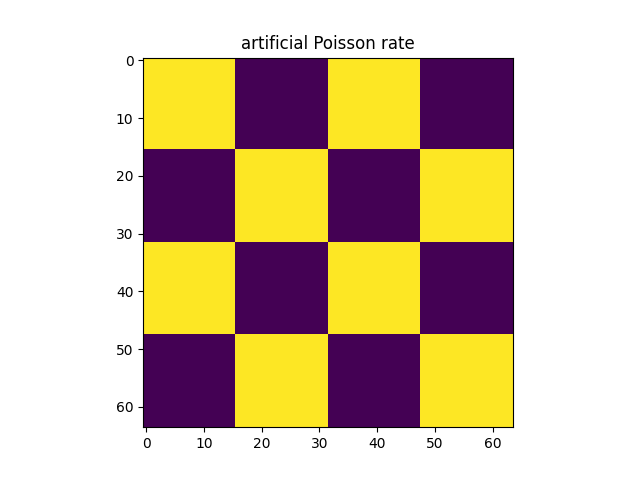
\includegraphics[width=0.72\textwidth]{figures/Figure_2.png}
\end{center}

Example I: checkerboard structure with two intensity levels.
\end{frame}

\begin{frame}{Discretization: From Point Events to Counts}
After discretization into grid cells:
\[
n_i = \#\{\text{events in cell } i\},
\qquad
n_i \sim \operatorname{Poisson}(\lambda_i)
\]

\begin{center}
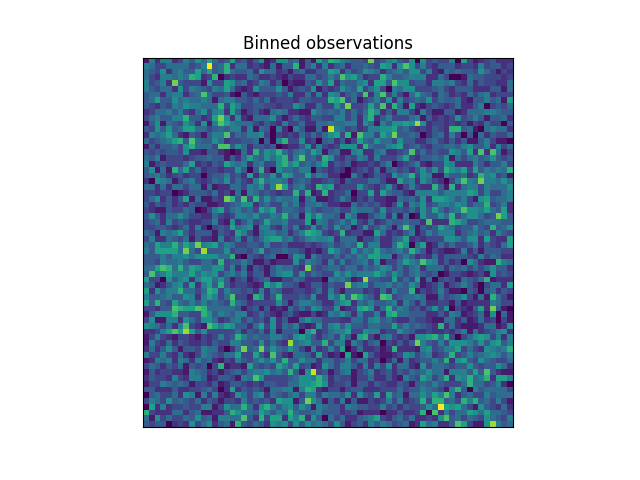
\includegraphics[width=0.70\textwidth]{figures/Figure_4.png}
\end{center}

The observations are discrete and noisy; the latent rate field is not observed.
\end{frame}

\begin{frame}{Synthetic Example II: A Second Realization}
\begin{columns}[T]
\begin{column}{0.49\textwidth}
\begin{center}
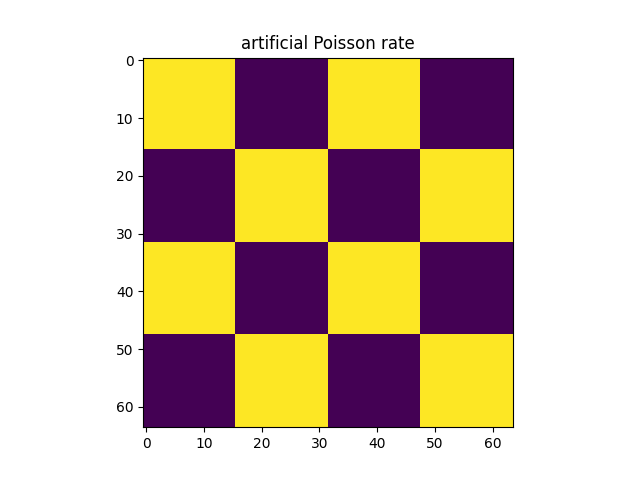
\includegraphics[width=\textwidth]{figures/Figure_9.png}

\scriptsize artificial Poisson rate
\end{center}
\end{column}
\begin{column}{0.49\textwidth}
\begin{center}
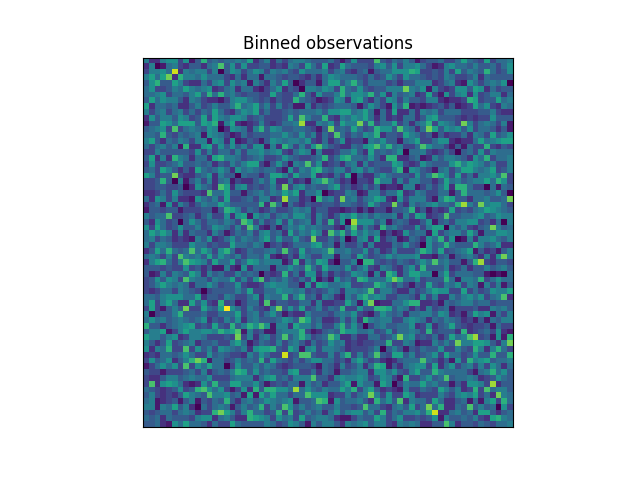
\includegraphics[width=\textwidth]{figures/Figure_11.png}

\scriptsize binned observations
\end{center}
\end{column}
\end{columns}

\medskip
Same generative mechanism, but a second synthetic data set for comparison.
\end{frame}

% -------------------------------------------------
\section{Bayesian Inference}

\begin{frame}{Posterior Target}
We want:
\[
p(f\mid n) \propto p(n\mid f)\,p(f)
\]

Likelihood:
\[
p(n_i\mid f_i)=\frac{(\lambda\sigmoid(f_i))^{n_i}}{n_i!}
\exp(-\lambda\sigmoid(f_i))
\]

Problem:
\begin{itemize}
\item nonlinear sigmoid term
\item no Gaussian conjugacy
\end{itemize}
\end{frame}

\begin{frame}{Poisson Splitting Trick}
Introduce latent counts:
\[
k_i \sim \operatorname{Poisson}(\lambda(1-\sigmoid(f_i)))
\]

Then the augmented likelihood can be rewritten in logistic form:
\[
p(n_i,k_i\mid f_i)
\propto
\frac{e^{n_i f_i}}{(1+e^{f_i})^{n_i+k_i}}
\]

This opens the door for P\'olya--Gamma augmentation.
\end{frame}

\begin{frame}{P\'olya--Gamma Augmentation}
Introduce:
\[
\omega_i \mid f_i \sim PG(b_i,f_i),
\qquad b_i=n_i+k_i
\]

Conditional on $\omega_i$:
\[
\log p(f_i\mid\omega_i)
=
-\frac12\omega_i f_i^2 + \kappa_i f_i + c
\]

Now the model becomes quadratic in $f$.
\end{frame}

\begin{frame}{Gaussian Conditional Posterior}
Combining with the Gaussian prior gives:
\[
f\mid n,k,\omega \sim \mathcal N(m,Q^{-1})
\]
with
\[
Q = \Sigma^{-1}+\Omega,
\qquad
\Omega=\operatorname{diag}(\omega_1,\dots,\omega_n)
\]

This is the key computational simplification.
\end{frame}

\begin{frame}{Efficient Sampling via Cholesky}
Instead of computing $Q^{-1}$ explicitly:
\[
Q = LL^\top
\]

Then solve triangular systems to sample from
\[
\mathcal N(m,Q^{-1})
\]

Main computational cost per Gibbs iteration:
\begin{itemize}
\item update latent variables
\item Cholesky factorization / linear solve
\end{itemize}
\end{frame}

% -------------------------------------------------
\section{Results}

\begin{frame}{Gaussian First Guess}
\begin{center}
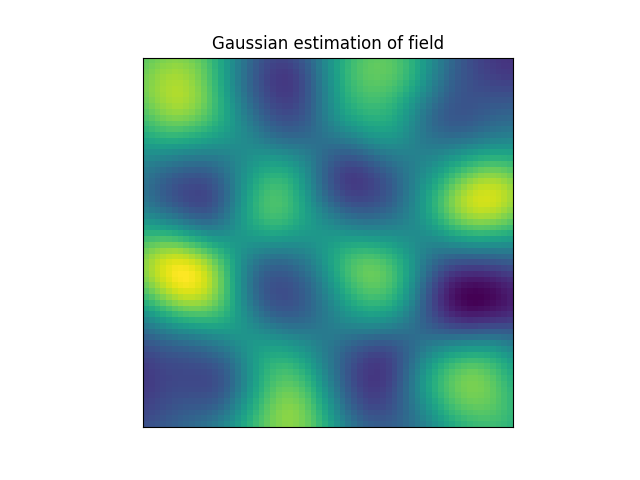
\includegraphics[width=0.72\textwidth]{figures/Figure_5.png}
\end{center}

Smooth initialization before full Gibbs sampling.
\end{frame}

\begin{frame}{Posterior Samples}
\begin{center}
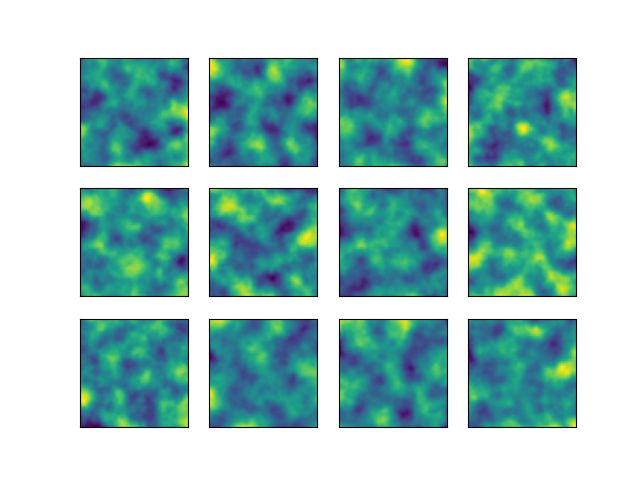
\includegraphics[width=0.82\textwidth]{figures/Figure_6.png}
\end{center}
\end{frame}

\begin{frame}{Posterior Mean Reconstruction: Example I}
\begin{center}
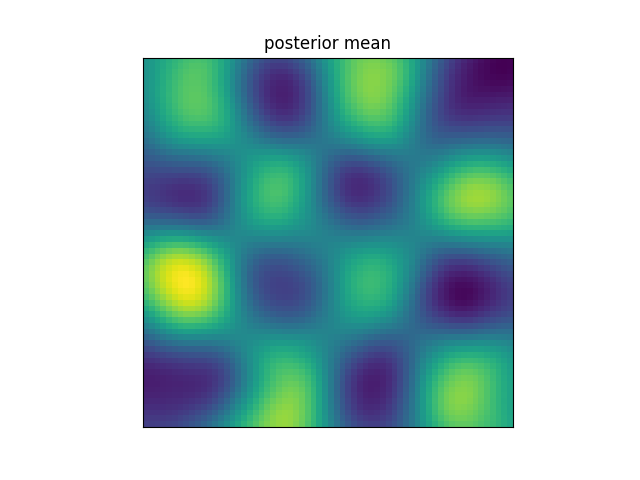
\includegraphics[width=0.72\textwidth]{figures/Figure_7.png}
\end{center}

Recovered spatial structure from event data.
\end{frame}

\begin{frame}{Posterior Mean Reconstruction: Example II}
\begin{center}
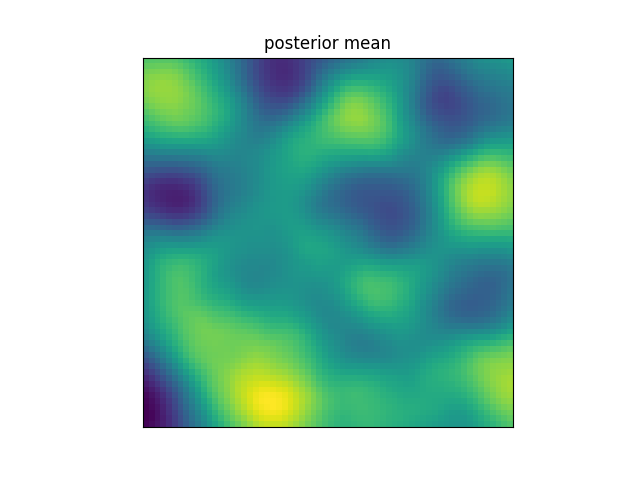
\includegraphics[width=0.72\textwidth]{figures/Figure_14.png}
\end{center}

The posterior mean is smoother than the discrete observations and reflects the spatial prior.
\end{frame}

\begin{frame}{Comparing the Two Synthetic Examples}
\begin{columns}[T]
\begin{column}{0.49\textwidth}
\begin{center}
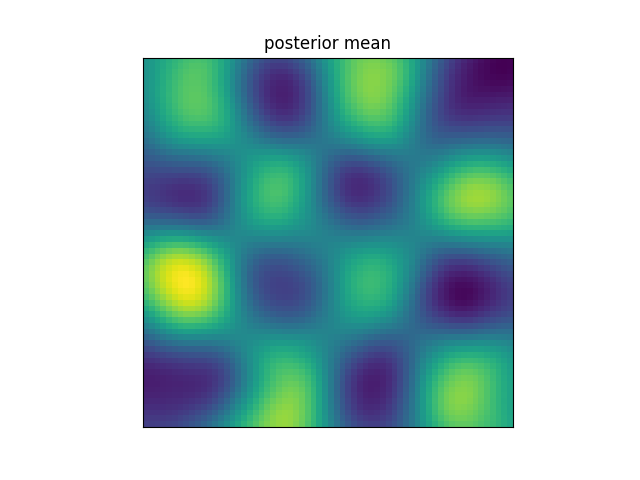
\includegraphics[width=\textwidth]{figures/Figure_7.png}

\scriptsize posterior mean, example I
\end{center}
\end{column}
\begin{column}{0.49\textwidth}
\begin{center}
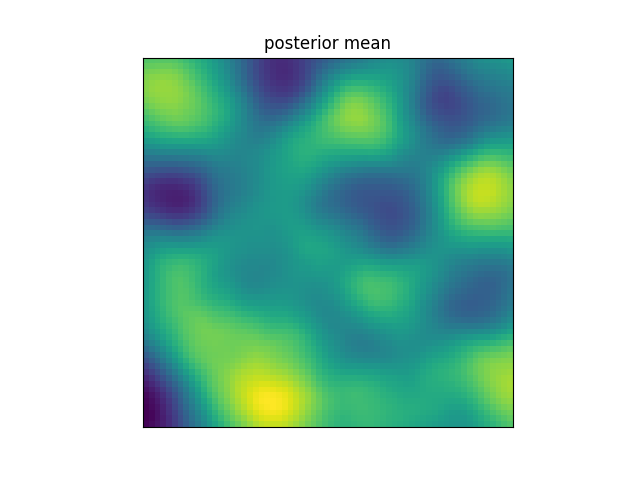
\includegraphics[width=\textwidth]{figures/Figure_14.png}

\scriptsize posterior mean, example II
\end{center}
\end{column}
\end{columns}

\medskip
Both reconstructions illustrate the same principle: noisy event counts are regularized through the latent Gaussian spatial model.
\end{frame}

% -------------------------------------------------
\section{Takeaways}

\begin{frame}{Takeaways}
\begin{itemize}
\item Point events can be modeled via latent spatial Poisson fields.
\item A Gaussian prior on $f$ induces flexible rate priors.
\item P\'olya--Gamma augmentation restores conditional Gaussian structure.
\item Gibbs sampling becomes efficient via Cholesky updates.
\item The framework extends naturally to real earthquake data and adaptive grids.
\end{itemize}
\end{frame}

\begin{frame}{Outlook}
Future directions:
\begin{itemize}
\item Quadtree / adaptive grids
\item Sparse precision matrices
\item Nonstationary covariance kernels
\item Real earthquake catalogs
\item Spatio-temporal extensions
\end{itemize}
\end{frame}

\begin{frame}{Thank you}
\begin{center}
\Large Thank you for your attention!\\[1em]
Questions?
\end{center}
\end{frame}

\begin{frame}{Limitations of the Sigmoid Link}
The sigmoid link is useful because it guarantees positivity and gives a tractable P\'olya--Gamma Gibbs sampler.

\medskip
However, it also introduces limitations:
\begin{itemize}
\item the intensity is bounded by the fixed scale parameter $\lambda$,
\[
0<\lambda_i<\lambda,
\]
\item large positive values of $f_i$ are compressed due to saturation,
\item the P\'olya--Gamma variables change in every iteration, so the Gaussian update requires repeated linear algebra,
\item the upper bound may be restrictive for data sets with strongly varying event rates.
\end{itemize}

\medskip
This motivates considering alternative positive link functions.
\end{frame}

\begin{frame}{Beyond the Sigmoid Link}
A natural next question is:
\[
\text{Can we keep positivity while avoiding the fixed upper bound?}
\]

\medskip
One possible alternative is the softplus / soft-ramp link:
\[
\lambda_i = \log(1+e^{f_i}).
\]

\medskip
It remains positive, but grows approximately linearly for large $f_i$.

\begin{block}{Next part}
Cristina presents an alternative inference strategy based on this softer, unbounded link function.
\end{block}
\end{frame}


% -------------------------------------------------
\appendix
\section{Appendix}

\begin{frame}{Appendix: Synthetic Example II -- Event Catalog}
\begin{center}
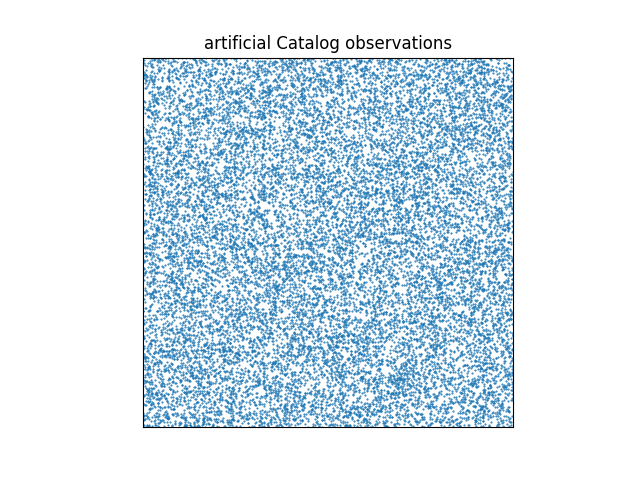
\includegraphics[width=0.72\textwidth]{figures/Figure_10.png}
\end{center}
\end{frame}

\begin{frame}{Appendix: Synthetic Example II -- Gaussian First Guess}
\begin{center}
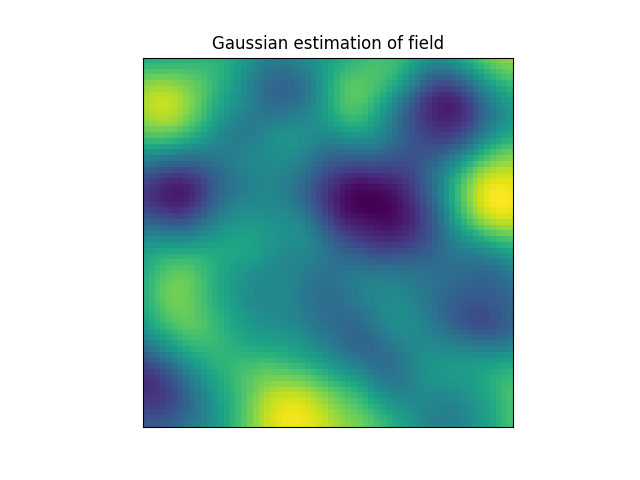
\includegraphics[width=0.72\textwidth]{figures/Figure_12.png}
\end{center}
\end{frame}

\begin{frame}{Appendix: Synthetic Example II -- Posterior Samples}
\begin{center}
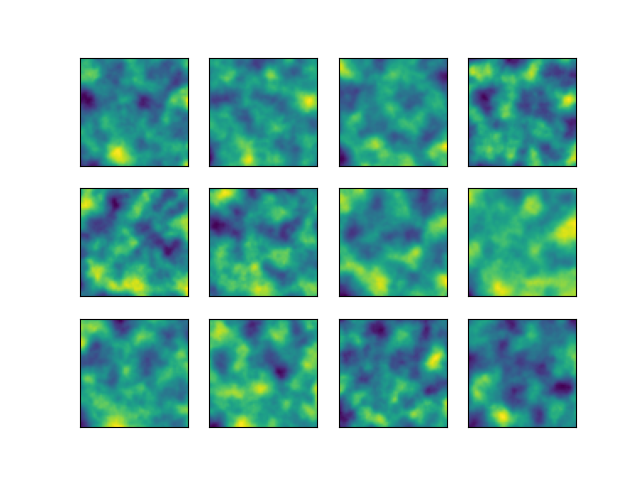
\includegraphics[width=0.82\textwidth]{figures/Figure_13.png}
\end{center}
\end{frame}

\begin{frame}{Appendix: Real Earthquake Data}
\begin{center}
bild aus habana exp quadtree
\end{center}

Possible discussion points:
\begin{itemize}
\item real point process data
\item spatially varying seismic activity
\item comparison with synthetic experiments
\end{itemize}
\end{frame}

\begin{frame}{Appendix: Adaptive Grid / Quadtree}
\begin{center}
bild aus habana exp quadtree
\end{center}

Possible discussion points:
\begin{itemize}
\item more cells where the data are dense
\item fewer cells where the data are sparse
\item rates must be interpreted relative to cell area
\end{itemize}
\end{frame}

\end{document}